\section{Introducción}

\subsection{DAOs y Blockchain}
\begin{frame}
    \begin{block}{Organización Autónoma Decentralizada (DAO)}
        Tipo de organización que permite la coordinación de proyectos mediante un proceso de \textbf{votación} democrático utilizando la tecnología \textbf{blockchain}\footnote{\textcite{hassan_decentralized_2021}}.
    \end{block}
\end{frame}

\begin{frame}
    \begin{figure}
        \centering
        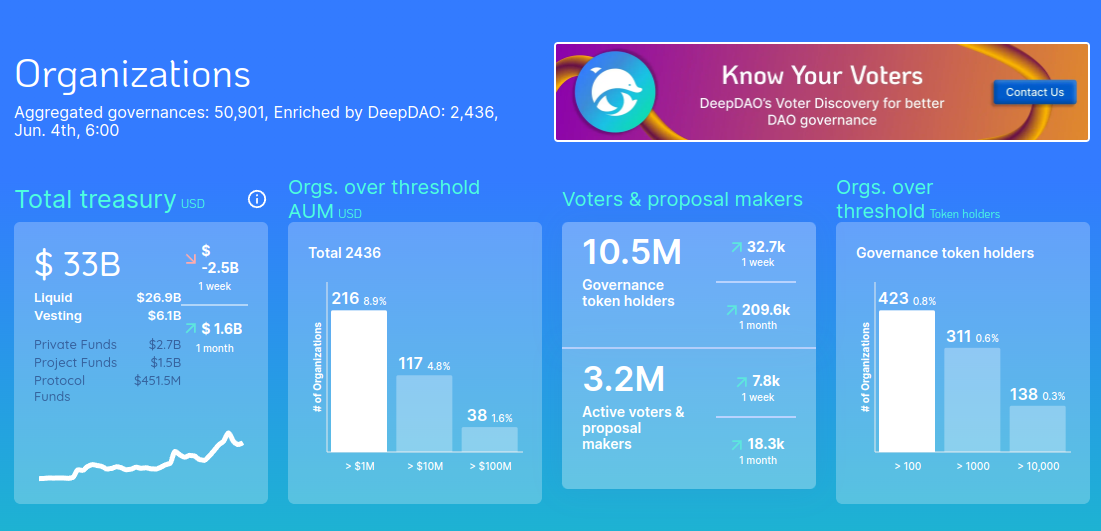
\includegraphics[height=50mm]{images/screenshots/Screenshot_20240604_172208.png}
        \caption{Captura de pantalla del portal de analíticas Deepdao\footnote{\url{https://deepdao.io/organizations}}}
        \label{fig:enter-label}
    \end{figure}
\end{frame}

\begin{frame}{Blockchain}
    % Poner una figura de ``el blockchain" (la cadena de bloques, que se vea coamo se enlazan los bloques, que tienen un hash, y poco más), y otra con como se distribuye en nodos
    \begin{figure}
        \centering
        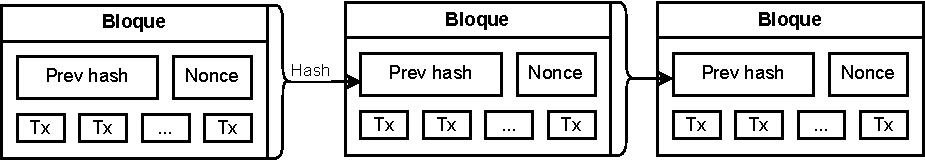
\includegraphics[width=\linewidth]{./images/diagrams/blockchain.drawio.pdf}
        \caption{Representación de una cadena de bloques}
    \end{figure}
\end{frame}

\begin{frame}
    \begin{figure}
        \centering
        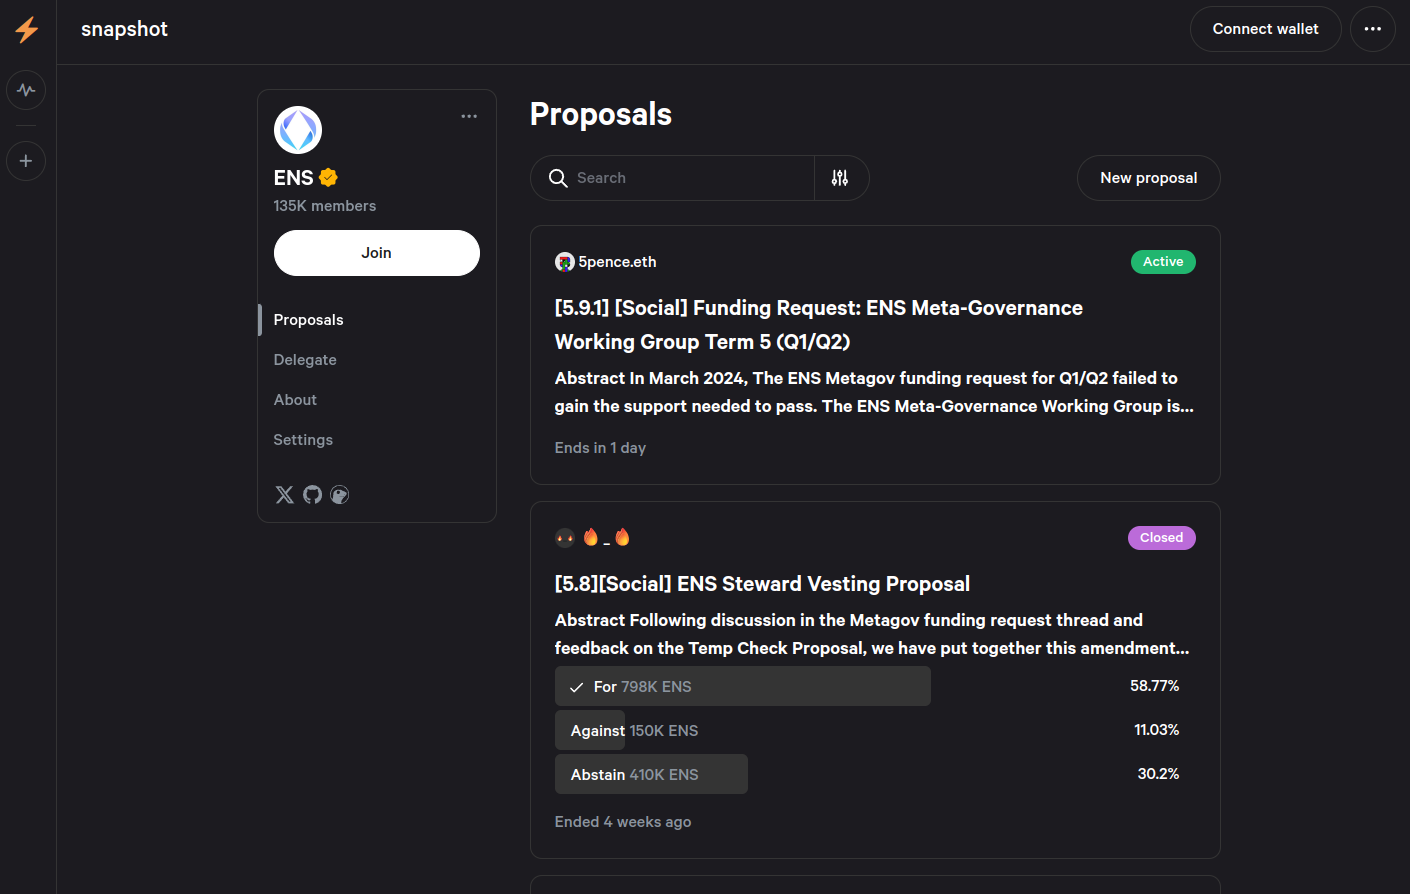
\includegraphics[width=87mm]{images/screenshots/Snapshot_ENS_Proposals.png}
        \caption{Captura de pantalla de la interfaz de votación de la DAO del protocolo ENS. \url{https://snapshot.org/\#/ens.eth}}
    \end{figure}
\end{frame}

\subsection{Motivación}

\begin{frame}
    \begin{itemize}[<+->]
        \item \textbf{Baja participación}: Menos de la mitad de usuarios han votado alguna vez\footnote{\footcite{arroyo_dao-analyzer_2022}}
        \item \textbf{Gran volumen de propuestas}: 150 propuestas/7 días en PancakeSwap o 70 en Decentraland\footnote{Notebook: \href{https://github.com/daviddavo/upm-tfm-notebooks/blob/main/04c_dao-census-onedao.ipynb}{04c\_dao-census-onedao.ipynb}}
        \item \textbf{Sin personalización}\footnote{\footcite{aviv_all_2023}}
    \end{itemize}
\end{frame}

\subsection{Sistemas Recomendadores}

\begin{frame}{DAOs y sistemas recomendadores}
    \begin{columns}
    \column{.5\textwidth}
        \begin{figure}
            \centering
            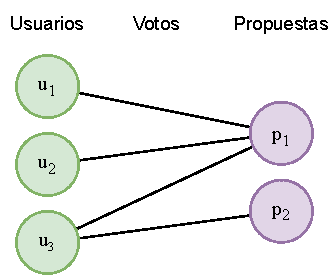
\includegraphics[height=44mm]{images/diagrams/dao-as-a-graph.drawio.pdf}
            \caption{Representación de una DAO como un grafo bipartito}
        \end{figure}
    \column{.5\textwidth}
        \begin{itemize}
            \item Usuarios
            \item Propuestas (\textit{ítems})
            \begin{itemize}
                \item \textbf{Descripción y texto}
                \item \textbf{Tiempo de apertura}
                \item \textbf{Tiempo de cierre}
            \end{itemize}
            \item Votos (\textit{Interacción})
            \begin{itemize}
                \item \textbf{Timestamp}
            \end{itemize}
        \end{itemize}
    \end{columns}

\end{frame}
